\prettypart{ВВЕДЕНИЕ}

В настоящее время возросшая скорость жизни как в её частных деталях, так и в общем, вынуждает человечество автоматизировать всё, что кажется возможным автоматизировать. Автоматизации подвергается как механическая деятельность человека --- промышленная революция, например ---, так и (особенно в последнее время вследствие общего увеличения доступных вычислительных мощностей) когнитивная деятельность человека.

Одной из идей, лежащих в основе механической автоматизации, является идея о создании роботов, выполняющих те или иные механические задачи.

Одной из идей, лежащих в основе когнитивной автоматизации, является идея об искусственном интеллекте, выполняющем те или иные интеллектуальные задачи.

Одной из задач, активно автоматизируемых в наши дни, является задача реализации образовательного процесса.

\chapter*{Рассуждения, приводящие к постановке\\ задачи ВКР}
Задача, сформулированная и решённая в выпускной квалификационной работе, поставлена на стыке нескольких технологически"=социальных явлений.

\section*{Доступная робототехника}
Развитию робототехники и, следовательно, образовательной робототехники значительно способствует снижение стоимости робототехнических решений начального уровня. В последние годы появилось большое количество микроконтроллеров и одноплатных компьютеров, позволяющих приобщиться к робототехнике большинству заинтересованных.

Набирает обороты движение <<мейкеров>>, использующих подручные и доступные средства для решения бытовых задач, творчества и развлечения на основе инженерного подхода.

% \subsection*{Популярные инструменты}
\label{popular-instruments}
Среди доступных элементов робототехники особенно заметны два класса устройств: микроконтроллеры и микрокомпьютеры.

Среди микроконтроллеров самыми популярными являются устройства семейства Arduino.

Среди микрокомпьютеров самыми популярными являются устройства семейства Raspberry Pi.

Оба семейства продуктов существуют достаточно долго, что привело к формированию сплочённого сообщества специалистов, что значительно снижает порог начала использования устройств: большая часть задач, интересных новичку, решена и разобрана в виде обучающего материала кем"=то в сети интернет.

\section*{Образовательная робототехника}
Образовательные технологии, как источник и следствие научного прогресса, находятся в постоянном развитии, постоянно влияя на общество. Текущее состояние образовательных технологий, направление их развития --- это наглядная демонстрация состояния и развития как общества, так и науки в наши дни.

% https://books.google.com/ngrams/graph?content=educational+robotics&case_insensitive=on&year_start=1980&year_end=2008&corpus=15&smoothing=3&share=&direct_url=t4%3B%2Ceducational%20robotics%3B%2Cc0%3B%2Cs0%3B%3Beducational%20robotics%3B%2Cc0%3B%3BEducational%20Robotics%3B%2Cc0
Сегодня одним из набирающих популярность направлений развития образовательных технологий является образовательная робототехника, что подтверждается исследованием корпусов Google Books English средствами Google Ngram \cite{google-ngram} по запросу $[\texttt{educational\ robotics}]$.


\begin{figure}[H]
\renewcommand\thefigure{0.1} % Make this Figure A
    \centering
    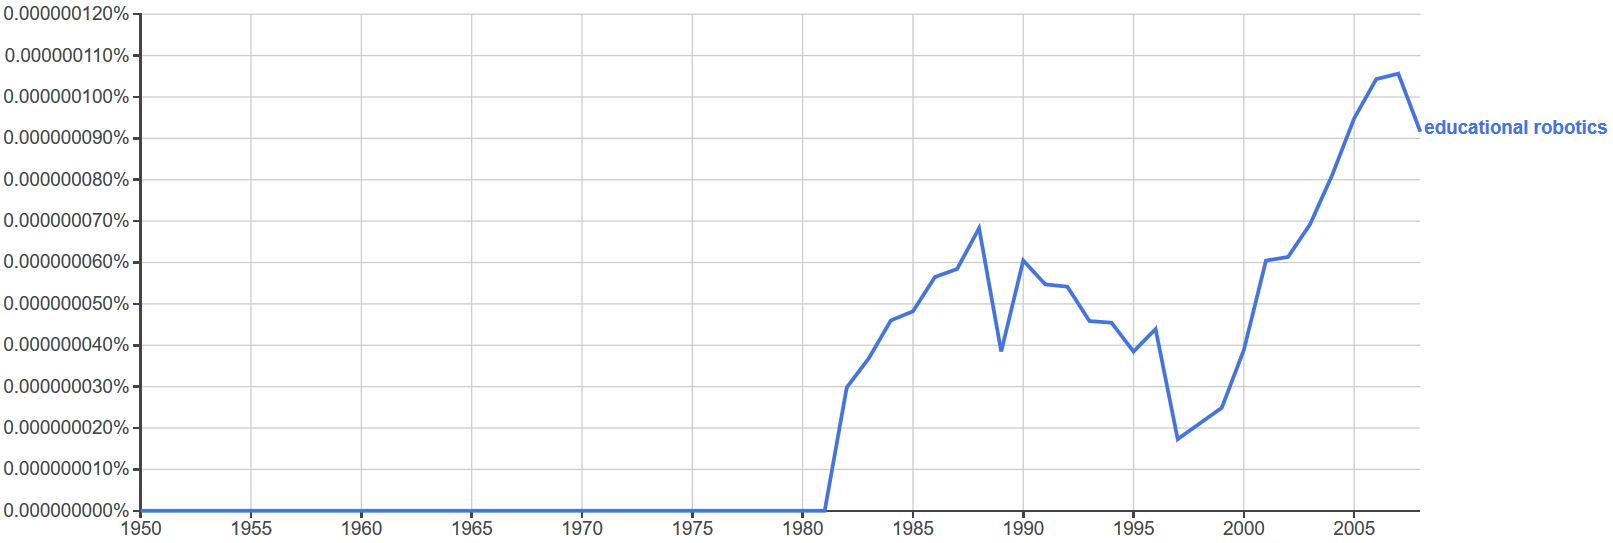
\includegraphics[scale=0.3]{images/ngram.png}
    \caption{Исследование корпуса Google Books English по запросу $[\texttt{educational\ robotics}]$}
    % \label{PO_scheme_img}
\end{figure}


\section*{Облачные технологии}
Автоматизация когнитивных задач в наше время требует значительных вычислительных мощностей, которые не всегда доступны локально. Это требование привело к повсеместному распространению облачных сервисов и <<тонких клиентов>>, позволяющих перенести вычислительно сложные задачи в облако.

Бывшие раньше уделом отдельных специалистов облачные технологии стали доступными любому любознательному энтузиасту --- так или иначе в повседневной деятельности облаками пользуется почти каждый, часто даже не подозревая об этом. Многие также используют облака для решения личных задач, например, для ведения семейного бюджета.

\chapter*{Постановка задачи, рассмотренной в ВКР}
Образовательная робототехника в наши дни набирает популярность, являясь фундаментальным инструментом современных образовательных технологий, требующих постоянного развития.

Робототехнические решения в последнее время получили значительное развитие и стали общедоступными.

Облачные сервисы, позволяющие реализовать как простые, так и самые сложные решения, используя последние достижения компьютерных наук, в последнее время перестали быть сложным малоизвестным инструментом и стали доступны и удобны.

Совокупность вышеприведённых фактов указывает на \textbf{актуальность следующей задачи}: создать и развить средства, позволяющие удобным образом создавать объекты образовательной робототехники, используя передовые технологии.

% \section*{Объект, предмет и цель работы}

В результате проведённого в рамках работы исследования существующих решений, относящихся к поставленной к задаче, популярных и набирающих популярность решений вспомогательных задач и подзадач основной задачи, были окончательно сформулированы объект, предмет и цель работы.

\textbf{Объект работы} --- когнитивный робот как единица образовательной робототехники.

\textbf{Предмет работы} --- реактивно"=делиберативный подход к созданию когнитивных роботов.

\textbf{Цель работы} --- разработка программно"=аппаратного комплекса для создания диалоговых когнитивных роботов на основе реактивно"=делиберативного подхода.